\section{Results}
\subsection{Budget Retention Reproduced an Operating Tradeoff}
\begin{table*}[t]
\centering
\footnotesize
\caption{Independent budget study: tighter retention ($.25-.50$), 16 paired demand days. Estimates and archived 95\% day-bootstrap intervals. Negative means lower.}
\label{tab:budget}
\setlength{\tabcolsep}{4pt}
\begin{tabularx}{\textwidth}{@{}lYYYY@{}}
\toprule
Comparison & Journey (s/person) & Readiness (s/trip) & Public delay (s/day) & Actual CV$^2$ \\
\midrule
Learned supervisor & \shortstack[r]{$-1.645$\\{\scriptsize $[-3.074,-0.070]$}} & \shortstack[r]{$-3.804$\\{\scriptsize $[-4.781,-2.915]$}} & \shortstack[r]{$-1001.62$\\{\scriptsize $[-1255.06,-771.75]$}} & \shortstack[r]{$+0.005646$\\{\scriptsize $[+0.003261,+0.009176]$}} \\[3pt]
Manual joint & \shortstack[r]{$-2.396$\\{\scriptsize $[-3.771,-0.976]$}} & \shortstack[r]{$-4.540$\\{\scriptsize $[-5.579,-3.595]$}} & \shortstack[r]{$-1185.44$\\{\scriptsize $[-1457.63,-939.62]$}} & \shortstack[r]{$+0.003025$\\{\scriptsize $[+0.001410,+0.004741]$}} \\[3pt]
\bottomrule
\end{tabularx}
\end{table*}

On the 16 independent days in Study~A, reducing retention from .50 to .25 lowered journey exposure and readiness delay under both learned and manual supervision (Table~\ref{tab:budget}). The learned controller's journey difference was $-1.645$ s/passenger, with interval $[-3.074,-0.070]$; the manual contrast was $-2.396$ s/passenger, with interval $[-3.771,-0.976]$. The corresponding actual CV$^2$ differences were positive for both controllers. The original budget-service proposition passed with its registered interpretation: improved passenger exposure and circulation accompanied by worse regularity.

These within-controller contrasts establish a configuration effect, not a learned-policy increment. In particular, manual joint also benefited from tighter retention. The public-delay and readiness columns describe related parts of the same vehicle-supply chain and are not independent replications of an operating benefit.

\begin{figure*}[t]
\centering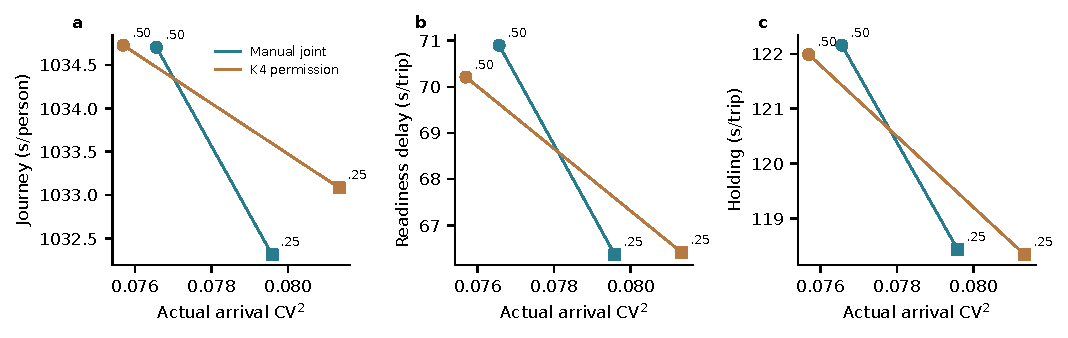
\includegraphics[width=\textwidth]{figures/budget_retention.pdf}
\caption{Budget retention and the service--circulation tradeoff on the same 16 independent demand days. Circles and squares denote retention .50 and .25, respectively. Each point is a complete-day mean; line segments connect only the two frozen settings and are not an optimized frontier. Reduced holding accompanies lower journey exposure and readiness delay but higher actual CV$^2$. Paired differences and uncertainty are reported in Table~\ref{tab:budget}.}
\label{fig:retention}
\end{figure*}

\subsection{Learning and Harmonic Inputs Had Different Evidence Boundaries}
\begin{table*}[t]
\centering
\footnotesize
\caption{Independent representation and supervisor comparisons, 16 paired demand days. K4 retains harmonics; K0 retains trend, online adaptation and innovation statistics. Intervals crossing zero are not equivalence tests.}
\label{tab:supervisor}
\setlength{\tabcolsep}{4pt}
\begin{tabularx}{\textwidth}{@{}lYYY@{}}
\toprule
Comparison & Journey (s/person) & Readiness (s/trip) & Actual CV$^2$ \\
\midrule
K4$-$manual, $\rho_B=.50$ & \shortstack[r]{$+0.022$\\{\scriptsize $[-0.608,+0.584]$}} & \shortstack[r]{$-0.690$\\{\scriptsize $[-1.400,-0.048]$}} & \shortstack[r]{$-0.000867$\\{\scriptsize $[-0.002202,+0.000353]$}} \\[3pt]
K4$-$manual, $\rho_B=.25$ & \shortstack[r]{$+0.773$\\{\scriptsize $[+0.075,+1.458]$}} & \shortstack[r]{$+0.045$\\{\scriptsize $[-0.620,+0.570]$}} & \shortstack[r]{$+0.001754$\\{\scriptsize $[-0.000713,+0.005083]$}} \\[3pt]
K4$-$K0, $\rho_B=.50$ & \shortstack[r]{$-0.562$\\{\scriptsize $[-1.567,+0.352]$}} & \shortstack[r]{$-0.104$\\{\scriptsize $[-0.597,+0.436]$}} & \shortstack[r]{$-0.000937$\\{\scriptsize $[-0.001668,-0.000175]$}} \\[3pt]
\bottomrule
\end{tabularx}
\end{table*}

At matched default retention, K4$-$manual journey exposure was $+0.022$ s/passenger with interval $[-0.608,0.584]$ (Table~\ref{tab:supervisor}). At $.25$, the difference was $+0.773$ s/passenger with interval $[0.075,1.458]$. Thus the independent panel did not establish a learned-supervisor journey advantage; the tighter setting favored the manual comparator on that endpoint. An interval spanning zero at the default setting did not establish equivalence.

The independent K4$-$K0 journey estimate was $-0.562$ s/passenger with interval $[-1.567,0.352]$, so the primary harmonic-journey proposition failed. The secondary actual-CV$^2$ interval favored K4 (Table~\ref{tab:supervisor}). These endpoints retain their separate status: the secondary regularity result does not replace the failed journey criterion.

Study~B produced the same executed policy as manual joint. Both newly trained learners selected joint at every one of their 47 publications in each of the 16 learned development paths. Their waiting, onboard, journey, readiness, public delay and CV$^2$ differences from manual joint were exactly zero at the matching retention on all four days. Each learner received 1,536 updates. The explicit-retention development screen therefore failed. Joint selection still invoked a demand- and vehicle-dependent timetable law; it did not imply a fixed timetable or an inactive controller.

\subsection{Pressure Credit Improved Delay but Failed Regularity Protection}
\begin{table*}[t]
\centering
\footnotesize
\caption{Pressure credit minus frozen simple-limit mixtures on 16 new paired demand days. Weights matched development holding exposure, not test-day holding or regularity. Both delay tests pass and both CV$^2$ protections fail.}
\label{tab:limits}
\setlength{\tabcolsep}{4pt}
\begin{tabularx}{\textwidth}{@{}lYYYY@{}}
\toprule
Comparison & Public delay (s/day) & Actual CV$^2$ & Journey (s/person) & Readiness (s/trip) \\
\midrule
Static trip credit & \shortstack[r]{$-3744.15$\\{\scriptsize $[-4401.41,-3025.06]$}} & \shortstack[r]{$+0.006573$\\{\scriptsize $[+0.004168,+0.008979]$}} & \shortstack[r]{$-4.761$\\{\scriptsize $[-6.670,-2.884]$}} & \shortstack[r]{$-14.354$\\{\scriptsize $[-16.858,-11.610]$}} \\[3pt]
Per-stop cap & \shortstack[r]{$-3123.80$\\{\scriptsize $[-3791.96,-2377.11]$}} & \shortstack[r]{$+0.006883$\\{\scriptsize $[+0.004661,+0.009121]$}} & \shortstack[r]{$-0.056$\\{\scriptsize $[-1.835,+1.849]$}} & \shortstack[r]{$-11.975$\\{\scriptsize $[-14.511,-9.145]$}} \\[3pt]
\bottomrule
\end{tabularx}
\end{table*}

On Study~C's 16 new days, pressure credit reduced public delay relative to both simple mixtures (Table~\ref{tab:limits}). The differences were $-3744.15$ s/day against static credit and $-3123.80$ s/day against the stop cap. Both delay bounds were below zero, but both actual-CV$^2$ intervals were above zero. Each joint gate failed under its original criterion.

The journey contrast against static credit was $-4.761$ s/passenger with interval $[-6.670,-2.884]$. Against the stop cap it was $-0.056$, with interval $[-1.835,1.849]$. Waiting intervals spanned zero for both families. Thus a passenger advantage was supported against one defined simple mixture, not uniformly against both.

Development exposure matching did not ensure matched test exposure. Pressure credit used 3.259 fewer holding seconds per trip than the static mixture and 1.797 fewer than the cap mixture on the new days. It improved delay on 16/16 and 15/16 days, respectively, while worsening CV$^2$ on 14/16 and 15/16 days. The failed protection was therefore directional across the panel, rather than driven by one adverse day.

\begin{figure*}[t]
\centering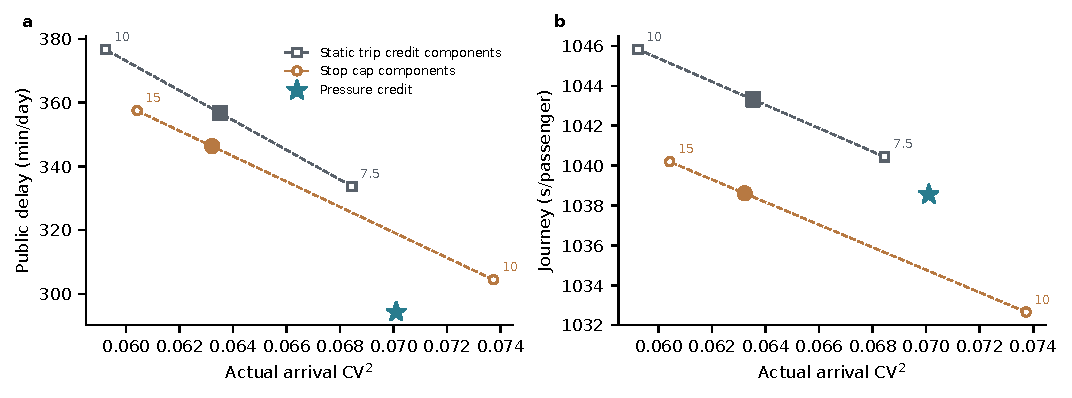
\includegraphics[width=\textwidth]{figures/independent_tradeoff.pdf}
\caption{Operating points on the original 16 independent days. Hollow points show the four frozen simple-limit components; filled points show their original ex-ante daily mixtures. Dashed segments span expectations of whole-day randomization, not mixing actions within a trip. Pressure credit lowers dispatch delay against both mixtures but increases CV$^2$. Component comparisons reveal a different delay--regularity geometry from the journey--regularity geometry. Paired mixture uncertainty is in Table~\ref{tab:limits}; these points are not a certified optimal frontier and no new mixture is selected.}
\label{fig:independent_tradeoff}
\end{figure*}

The finite calibration grid (Supporting Fig.~S1) and the independent operating points (Fig.~\ref{fig:independent_tradeoff}) answer different questions. The grid contains promising pressure-credit configurations on consumed development days, but does not certify a frontier on unseen days. The unchanged independent mixtures expose the resulting regularity cost without test-day intensity matching.

Reporting the four component policies also reveals why actual holding alone does not order the outcomes. Against the 10-s stop cap, pressure used 14.210 more holding seconds per trip while reducing public delay by 608.94 s/day and actual CV$^2$ by 0.003636; journey exposure increased by 5.900 s/passenger. Against the 7.5-s static setting, pressure also used more holding, but lowered journey and delay while the CV$^2$ interval crossed zero. Against the two looser components, pressure reduced holding and delay but worsened CV$^2$. These secondary contrasts are reported together in the Supporting Information. They distinguish operating dimensions without selecting a new mixture or overturning the original joint failures.

\subsection{Joint Credit and Operating Cost}
\begin{table*}[t]
\centering
\footnotesize
\caption{Common-reference joint-credit candidate minus each comparator on four NEW development days. Intervals are descriptive. This is not independent confirmation. Both simple-control delay screens fail; both mean CV$^2$ protections pass.}
\label{tab:joint}
\setlength{\tabcolsep}{4pt}
\begin{tabularx}{\textwidth}{@{}lYYYY@{}}
\toprule
Comparison & Public delay (s/day) & Actual CV$^2$ & Journey (s/person) & Holding (s/trip) \\
\midrule
Static mixture & \shortstack[r]{$+5917.10$\\{\scriptsize $[+3715.79,+8773.66]$}} & \shortstack[r]{$-0.013690$\\{\scriptsize $[-0.016188,-0.009969]$}} & \shortstack[r]{$+6.803$\\{\scriptsize $[+0.889,+15.613]$}} & \shortstack[r]{$+22.333$\\{\scriptsize $[+18.603,+26.062]$}} \\[3pt]
Stop-cap mixture & \shortstack[r]{$+6165.45$\\{\scriptsize $[+4157.09,+8765.84]$}} & \shortstack[r]{$-0.012680$\\{\scriptsize $[-0.016640,-0.008721]$}} & \shortstack[r]{$+10.744$\\{\scriptsize $[+4.138,+20.729]$}} & \shortstack[r]{$+24.454$\\{\scriptsize $[+21.333,+27.574]$}} \\[3pt]
Old pressure & \shortstack[r]{$+9918.50$\\{\scriptsize $[+6623.00,+13315.00]$}} & \shortstack[r]{$-0.020795$\\{\scriptsize $[-0.032846,-0.012465]$}} & \shortstack[r]{$+12.768$\\{\scriptsize $[+1.377,+25.861]$}} & \shortstack[r]{$+26.250$\\{\scriptsize $[+19.585,+32.352]$}} \\[3pt]
\bottomrule
\end{tabularx}
\end{table*}

The Study~D candidate improved actual CV$^2$ against both simple mixtures on all four new development days (Table~\ref{tab:joint}). However, journey exposure and public delay were worse on every day against each mixture. The mean-delay conditions failed and both mean-CV$^2$ protections passed; the overall development screen failed.

The execution record showed 985 evaluated credit requests: 34 were admitted, 919 offered no joint improvement under the common reference, and 32 had an unsupported reference. All admitted budgets passed chronological accounting. Actual holding averaged 146.594 s/trip, compared with 120.344 for old pressure. Relative to old pressure, the candidate's CV$^2$ decreased by 0.020795, while journey exposure increased by 12.768 s/passenger and public delay increased by 9918.50 s/day. The candidate was closed without changing its constraints or opening independent confirmation.

\subsection{Operating Conditions Separate Budget and Timetable Effects}
\begin{table*}[t]
\centering\footnotesize
\caption{Conditional timetable and budget effects on four new paired demand days per regime. Timetable means joint minus budget-only; budget means joint minus timetable-only. Day-bootstrap intervals are descriptive, not a replacement for the original confirmation gates.}
\label{tab:factorial}
\setlength{\tabcolsep}{4pt}
\begin{tabularx}{\textwidth}{@{}llYYYY@{}}\toprule
Regime & Added component & Journey (s/person) & Public delay (min/day) & Readiness (s/trip) & Actual CV$^2$ \\ \midrule
nominal & Timetable given budget & \shortstack[r]{$+2.013$\\{\scriptsize $[+0.886,+3.847]$}} & \shortstack[r]{$+3.41$\\{\scriptsize $[+0.53,+6.29]$}} & \shortstack[r]{$+0.33$\\{\scriptsize $[-0.47,+1.12]$}} & \shortstack[r]{$+0.001951$\\{\scriptsize $[+0.000400,+0.003502]$}} \\[2pt]
nominal & Budget given timetable & \shortstack[r]{$-6.887$\\{\scriptsize $[-10.587,-0.817]$}} & \shortstack[r]{$-142.58$\\{\scriptsize $[-157.00,-128.17]$}} & \shortstack[r]{$-32.69$\\{\scriptsize $[-36.10,-29.28]$}} & \shortstack[r]{$+0.032276$\\{\scriptsize $[+0.026438,+0.037888]$}} \\[2pt]
light & Timetable given budget & \shortstack[r]{$+0.951$\\{\scriptsize $[-0.257,+2.408]$}} & \shortstack[r]{$+9.70$\\{\scriptsize $[+5.68,+14.62]$}} & \shortstack[r]{$+1.62$\\{\scriptsize $[+0.66,+2.83]$}} & \shortstack[r]{$+0.002047$\\{\scriptsize $[-0.000720,+0.005999]$}} \\[2pt]
light & Budget given timetable & \shortstack[r]{$-4.005$\\{\scriptsize $[-5.755,-1.853]$}} & \shortstack[r]{$-115.64$\\{\scriptsize $[-162.07,-73.84]$}} & \shortstack[r]{$-26.56$\\{\scriptsize $[-37.16,-17.05]$}} & \shortstack[r]{$+0.026161$\\{\scriptsize $[+0.011042,+0.050500]$}} \\[2pt]
heavy & Timetable given budget & \shortstack[r]{$-0.369$\\{\scriptsize $[-0.726,-0.069]$}} & \shortstack[r]{$+1.23$\\{\scriptsize $[+0.73,+1.95]$}} & \shortstack[r]{$-0.10$\\{\scriptsize $[-0.25,+0.07]$}} & \shortstack[r]{$+0.000629$\\{\scriptsize $[-0.000191,+0.001843]$}} \\[2pt]
heavy & Budget given timetable & \shortstack[r]{$-29.699$\\{\scriptsize $[-42.137,-20.531]$}} & \shortstack[r]{$-275.40$\\{\scriptsize $[-318.79,-231.33]$}} & \shortstack[r]{$-63.22$\\{\scriptsize $[-73.19,-53.07]$}} & \shortstack[r]{$+0.023173$\\{\scriptsize $[+0.018793,+0.028463]$}} \\[2pt]
rushshift & Timetable given budget & \shortstack[r]{$+1.217$\\{\scriptsize $[+0.037,+2.523]$}} & \shortstack[r]{$+5.25$\\{\scriptsize $[+0.78,+10.28]$}} & \shortstack[r]{$+0.76$\\{\scriptsize $[-0.23,+1.95]$}} & \shortstack[r]{$-0.000076$\\{\scriptsize $[-0.000725,+0.000574]$}} \\[2pt]
rushshift & Budget given timetable & \shortstack[r]{$-20.186$\\{\scriptsize $[-31.214,-12.149]$}} & \shortstack[r]{$-175.49$\\{\scriptsize $[-239.82,-138.47]$}} & \shortstack[r]{$-40.28$\\{\scriptsize $[-55.17,-31.70]$}} & \shortstack[r]{$+0.021655$\\{\scriptsize $[+0.016825,+0.025009]$}} \\[2pt]
\bottomrule\end{tabularx}
\end{table*}

Study~E completed all 144 paired paths. Relative to fixed360 with native bilateral holding, joint pressure control reduced journey exposure by 12.204, 6.841, 27.557 and 22.340 s/passenger under nominal, light, heavy and rush-shift demand, respectively (Fig.~\ref{fig:conditions}). Readiness delay fell by 37.57, 27.52, 60.26 and 43.58 s/trip. In all four regimes, however, actual CV$^2$ increased: the corresponding differences were 0.031353, 0.023641, 0.023758 and 0.020365. These are service--circulation gains accompanied by reduced regularity, not joint dominance.

\begin{figure*}[t]
\centering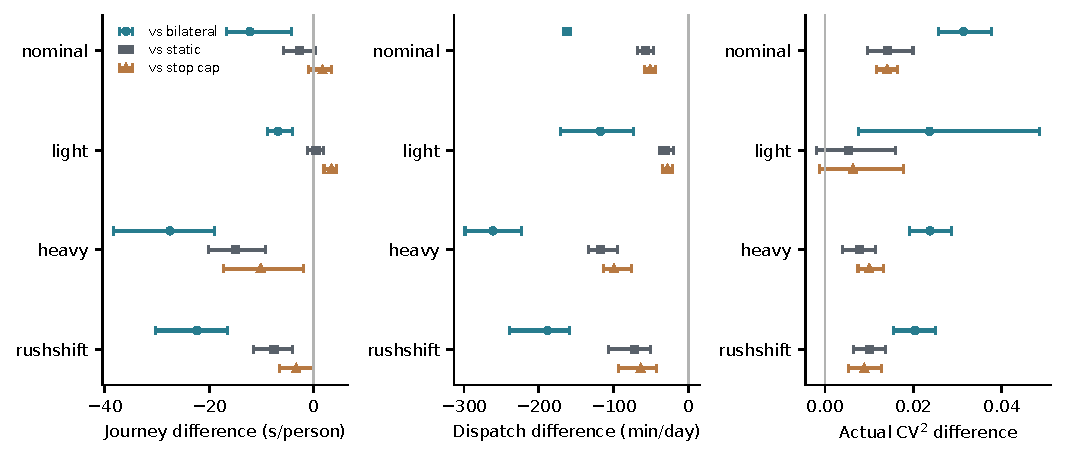
\includegraphics[width=\textwidth]{figures/regime_robustness.pdf}
\caption{Joint pressure control minus the native fixed360 bilateral baseline and the two frozen simple-limit mixtures under four operating conditions. Each estimate uses four independent paired demand days. Intervals are descriptive day bootstraps. No mixture or controller is selected from this panel. The CV$^2$ cost persists against native bilateral in every regime.}
\label{fig:conditions}
\end{figure*}

The model-controller factorial identifies pressure credit as the principal source of the circulation savings (Table~\ref{tab:factorial}). Adding the timetable law to budget-only control increased journey exposure by 2.013 s/passenger under nominal demand, 0.951 under light demand and 1.217 under rush shift; under heavy demand it reduced exposure by 0.369 s/passenger. The conditional timetable effect on public delay was adverse in all four regimes: $+204.5$, $+582.0$, $+74.0$ and $+314.75$ s/day. Active plan changes therefore did not establish a consistent incremental timetable benefit. All four corners and the interaction estimates are retained in the Supporting Information.

The original simple-mixture tradeoff also changed with operating conditions. Pressure lowered public delay relative to both mixtures in every regime. Journey exposure was worse than the stop-cap mixture in light demand by 3.423 s/passenger, with descriptive interval $[1.993,4.475]$, while heavy and rush-shift means favored pressure. Against the individual 10-s cap, the original panel's favorable delay--regularity combination did not recur uniformly: nominal CV$^2$ increased by 0.006184, whereas light CV$^2$ decreased by 0.008195 but journey exposure increased by 6.089 s/passenger. Reporting all components avoids interpreting one favorable projection as a general frontier improvement.

\subsection{Executed Supply Chains and Passenger Distribution}
The preregistered vehicle example was trip 31 of bus 9 on the first nominal day (Fig.~\ref{fig:chain}). Fixed-model and timetable-only control executed 105 s of holding, returned at 7616 s and launched the same vehicle on trip 42 at 7617 s. Budget-only and joint control executed 70 s, returned at 7585 s and launched at 7586 s. Thus a 35-s command reduction coincided with a 31-s earlier return and following departure; the timetable law added no change on this chain. The example demonstrates physical propagation under the frozen policies, rather than an isolated causal effect of holding with all subsequent states fixed.

\begin{figure*}[t]
\centering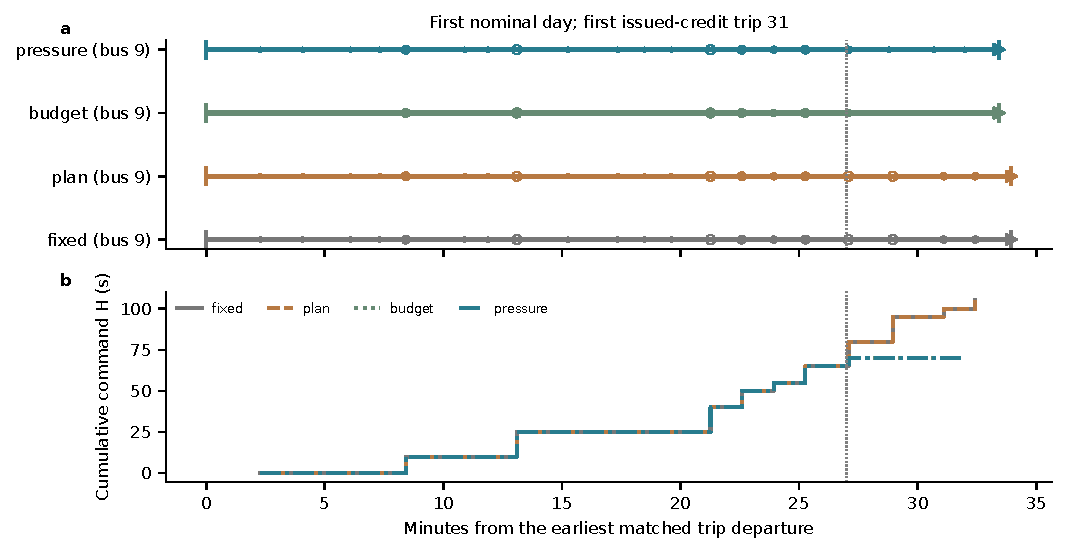
\includegraphics[width=.95\textwidth]{figures/vehicle_time_chain.pdf}
\caption{The predeclared first issued-credit trip on the first nominal day. Top: departure, physical return (right tick), and the assigned vehicle's next departure (triangle). Circles mark command submission times, with area increasing with holding. Bottom: cumulative commanded holding, all verified executed. The dotted line is the first credit publication. Fixed and plan-only coincide here, as do budget-only and joint. Future vehicle identities are evaluation labels, not controller inputs.}
\label{fig:chain}
\end{figure*}

Timetable revisions did reach execution elsewhere. On the four nominal days, joint had 19, 27, 26 and 20 revised final releases; 18, 26, 25 and 20 departures occurred exactly at those releases. Relative to budget-only, 75, 97, 72 and 57 actual departure times changed. This execution evidence excludes an inactive timetable as the explanation for its weak conditional result; it does not turn those changes into passenger gains. Trip/hour and same-vehicle-chain readouts are included with the source data.

Joint control reduced each day's journey P95 relative to native bilateral on average by 42.45, 17.92, 112.34 and 84.84 s across the four regimes. Mean gains did not benefit every cohort: on nominal days, several early origin stations had higher journey exposure despite the aggregate improvement (Supporting Information). Relative to the stop-cap mixture, light-demand journey P95 increased by 7.10 s, with descriptive interval $[2.91,11.28]$. These distributional results retain daily percentiles and passenger-weighted cohort means as distinct estimands.

Public-delay savings also coexisted with early departures. Joint averaged 7.00, 3.25, 9.75 and 5.00 early trips/day, with summed earliness of 15.75, 10.00, 33.25 and 10.50 s/day. Earliness is reported separately, not canceled against lateness. All vehicles completed their trips and no passengers remained onboard at the endpoint. Mean unserved counts were 0.50, 1.00, 744.75 and 47.00 passengers/day, respectively, with their fixed-horizon waiting retained; heavy-demand tail results therefore concern a capacity-stressed system rather than universal passenger completion.

\subsection{Engineering Validity and Computation}
All 80 Study~C test paths and all 24 Study~D development paths completed with the fixed fleet, full trip roster and valid physical accounting. The Study~D implementation also exactly reproduced the archived pressure path and its no-proposal selector path, with zero diagnostic roundoff in the registered comparison. One zero-traffic test-fixture failure was repaired and retained; it did not consume a traffic path. These checks support execution validity, separately from the scientific outcomes.

Archived full-day wall time in Study~C had median 21.26 min and maximum 29.35 min. In Study~D the corresponding values were 24.36 and 27.27 min, with 24 development paths running concurrently on Linux CPU nodes. These are batch experiment costs under the recorded server workloads, not per-query real-time latency guarantees.

Study~E used 146 charged starts: 144 successful formal paths and two old-day engineering attempts, including one preserved failed observation capture. The repaired engineering path exactly reproduced its archive. All formal paths ran from the standalone source snapshot. Their wall times had median 19.93 min, 95th percentile 26.87 min and maximum 28.78 min; native bilateral timings include passive graph observation. Across paths, the individual callback P95 ranged from 0.061 to 0.713 s. Queue and result-transfer time are excluded, and these observations do not guarantee one-second real-time execution.

Graph support averaged 85.70\%, 95.21\%, 0\% and 60.62\% under nominal, light, heavy and rush-shift demand. Under heavy demand, every query used native-rule fallback, still projected onto any remaining issued credit. Its 2,833 changes to native requests were budget projections rather than supported graph optima. The heavy-demand service gains cannot therefore be attributed to model-based action optimization. The primary exposure uses the frozen one-second occupancy integral; timestamp-based passenger readouts differed by about half a second per passenger, with paired offsets below $6\times10^{-12}$ s and no effect on the primary contrasts.
